\documentclass[12pt] {article}
\usepackage{times}
\usepackage[margin=1in,bottom=1in,top=1in]{geometry}

\usepackage{hhline}
\usepackage{subfig}
\usepackage{amsmath}
\usepackage[inline,shortlabels]{enumitem}%enumerate with letters
\usepackage[square,numbers]{natbib}
\usepackage{graphicx}
\bibliographystyle{unsrtnat}
\begin{document}

\title{Assignment Three -  EEC254}
\author{Ahmed H. Mahmoud}
\date{February 6th, 2018}
\maketitle

%============Table========
%\begin{figure}[tbh]
% \centering    
%\begin{tabular}{ |p{4cm}|| p{2cm}|p{2cm}|p{2cm}|p{2cm}|}
% \hline
% & Processor 1 &  Processor 2  & Processor 3 & Processor 4\\ \hhline{|=|=|=|=|=|}
% \hline
% Performance          &$1.08$        &$1.425$       &\textbf{1.52}  &   \\
% \hline
%\end{tabular} 
%\caption{Metric table for the four processors}
%   \label{tab:metric}
%\end{figure} 
%============Figure========
%\begin{figure}[!tbh]
%\centering        
%   \subfloat {\includegraphics[width=0.65\textwidth]{fig2_4.png}}
%   \caption{ }
%   \label{fig:fig}
%\end{figure}

%\begin{enumerate}[(a)]
%\end{enumerate}


\paragraph{Problem 4.1:} 
Figure~\ref{fig:fig41} shows a sketch of the feasible set given the problem's constraints. The feasible set can be define mathematically as the convex hull of the following points (each point is expressed as $(x_1,x_2)$): $(0,\infty), (0,1), (0.4,0.2), (1,0)$ and $(0,\infty)$
\begin{figure}[!tbh]
\centering        
   \subfloat {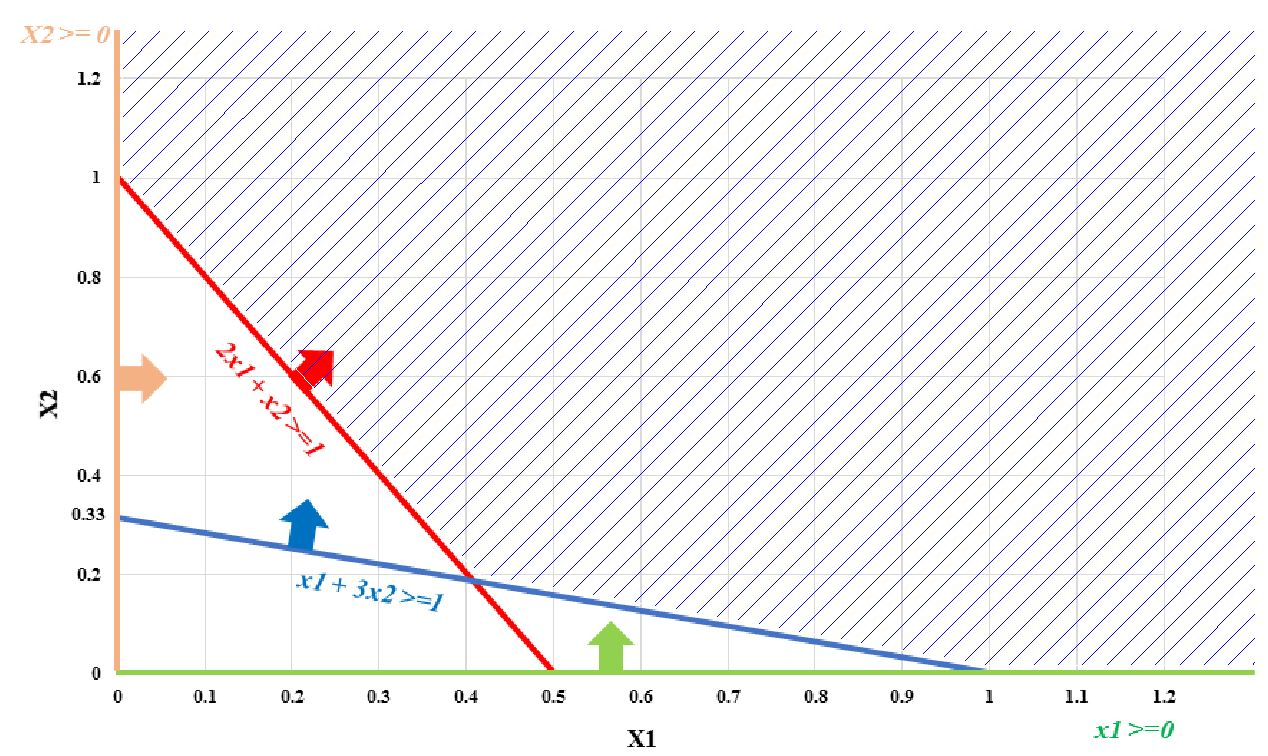
\includegraphics[width=0.5\textwidth]{4_1.jpg}}
   \caption{Sketch of the feasible set of the constraints in Problem 4.1. Notice that it is an open region.}
   \label{fig:fig41}
\end{figure}

The optimal set and optimal value for the given objective functions are:
\begin{enumerate} [(a)]
\item One point $x^{*}=(0.4,0.2)$, with optimal value $p^{*} = 0.6$
\item The problem is unbounded below
\item The optimal set is the ray starting from point $(0,1)$ and goes to infinity in the positive $x_2$ direction. Thus, $X_{opt}= \left\lbrace(x_{1},x_{2})| x_{1} = 0, x_{2}\geq 1 \right\rbrace$. The optimal value $p^{*}=0$. 
\item One point $x^{*}=(\frac{1}{3},\frac{1}{3})$, with optimal value $p^{*} = \frac{1}{3}$
\item One point $x^{*}=(0.5,\frac{1}{6})$, with optimal value $p^{*} = 0.5$
\end{enumerate}

\paragraph{Problem 4.3:} 
In order to apply the optimality criterion on the give function, we need to calculate gradient of the objective function. The objective function can be rewritten as 
\[
f = (\frac{1}{2})x^{T}Px + q^{T}x + r
\]

\[
f =
(\frac{1}{2}) 
\left[
\begin{array}{ccc}
x_1  & x_2 & x_3\\
\end{array} 
\right]
\left[
\begin{array}{ccc}
13  & 12 & -2\\
12  & 17 & 6\\
-2  & 6 & 12\\
\end{array} 
\right]
\left[
\begin{array}{c}
x_1  \\
x_2  \\
x_3\\
\end{array} 
\right]
 + 
\left[
\begin{array}{ccc}
-22  & -14.5 & 13\\
\end{array} 
\right]
+
\left[
\begin{array}{c}
x_1  \\
x_2  \\
x_3\\
\end{array} 
\right]
+1
\] 

\[
f = \frac{1}{2}(13x^{2}_{1}+17x^{2}_{2}+12x^{2}_{3} +24x_{1}x_{2}-4x_{1}x_{3}+12x_{2}x_{3})-22x_{1}-14.5x_{2}+13x_{3}+1
\]
Thus, the gradient is 
\[
\nabla f = 
\left[
\begin{array}{c}
13x_1+12x_2-2x_3-22  \\
17x_2 +12x_1+6x_3-14.5  \\
12x_3-2x_1+6x_2+13\\
\end{array} 
\right]
\]
Evaluating the gradient at $x^{*}=(1,\frac{1}{2},-1)$ gives 

\[
\nabla f (x^{*})= 
\left[
\begin{array}{c}
  -1\\
   0\\
   2\\
\end{array} 
\right]
\]

The optimality criterion is $\nabla f(x^{*})^{T}(y-x) \geq 0 $ for all $y$ and $x$ in the feasible set. Applying this criterion using the calculated gradient at $x^{*}$ gives 
$$
\nabla f(x^{*})^{T}(y-x) = -1(y_1-1) + 2(y_{3}+1)
$$
Using brute-force-style search for many different values of $y_{1}$ and $y_{3}$ between -1 and 1, we can verify that the above equation is always greater or equal to zero. 

\paragraph{Problem 4.8:} 
\begin{enumerate}[(a)]
%https://math.stackexchange.com/questions/319772/linear-optimization-problem-minimizing-a-linear-function-over-an-affine-set
\item $x$ should be on the range of $A$ in order for $Ax=b$ to be achieved. Thus, if $Ax=b$ has no solution then the optimal value is $\infty$. The other extreme case occurs if $c$ is not orthogonal to the null-space of $A$; (geometrically speaking) has some general position. This means we can decompose $c$ into two components; one that lies on the range of $A$ and the other one on the null space of $A$. The $c$ component on the null-space of $A$ will goes to zero since $x$ is in the range of $A$. The component of $c$ on the range of $A$ (more rigorously the result of dot product of $x$ and the component of $c$ on the range of $A$) is unbounded; it can keep decreasing forever. Thus, the optimal solution for when $c$ is not on the range of $A$ is $-\infty$. 

The special case where $c$ is in the range of $A$ can be written as $c = A^{T}\lambda$ for some vector $\lambda$. Since $x$ must satisfy $Ax=b$, we can plug in the $c = A^{T}\lambda$ into the objective function and get the solution as $\lambda^{T}b$ which is the optimal constant solution. 

\item Following the same reasoning we made in (a), the problem is unbounded below if $c$ is in a general position i.e, its has a non-zero component along the null-space of $A$. When $c$ is on the range of $A$, we can obtain an optimal solution by plugging in $c$ such that $c = A^{T}\lambda$ for some vector $\lambda$ in the objective function. The optimal solution is then $\lambda b$ for some $\lambda \leq 0$. We have to have $\lambda \leq 0$ because for positive $\lambda$ the problem will be unbounded below since we can keep decreasing the objective function forever. 

\item The objective function is dot product between two vectors. Thus, to minimizing it means minimizing each component contributes to the dot product. Since $x$ is inside a rectangle, then each of the component of $x$ should be on the boundary of that rectangle in order to obtain minimize the objective function. This will only depends on the sign of the $c$ component by which the $x$ component is multiplied. We should seek always $x$ that give negative value of its preservative component in the dot product. 
\item We can write the objective function as $c_{0}x_{0}+c_{1}x_{1}+c_{2}x_{2}\cdots $ and it is subject to $x_{0}+x_{1}+x_{2} \cdots = 1$ for all $x_{i}\geq 0$. Take $i=2$, this means we the objective function is a line and the optimal solution is one end of this line segment; the least of $c_{0}$ and $c_{1}$. In general case, the optimal solution is the minimum $c_{i}$ in the $c$ vector. 
\item Following similar logic we made in (d), the sum of $x$ elements is $\alpha$ and all elements should be between 0 and 1. Since $\alpha$ is integer, then some of the elements of $x$ should be zero in order to meat the constraints (otherwise $1^{T}x$ will be greater than $\alpha$. Other elements in $x$ should be ones for the same reasons. The number of elements of $x$ with one value should be equal to $\alpha$ value to minimize the objective function. This is the optimal solution.
\item 
\end{enumerate}
\paragraph{Problem 4.11:} 
Here the \textbf{Explanation} part is given such that if we make the argument that our LP reformulation is equivalent to the given problem, then that is means the optimal solution of the LP problem is equivalent to the optimal solution to the given problem. 
\begin{enumerate}[(a)]
\item \textbf{Formulation:} This minimization problem can be re-written as minimizing $t$ subject to $Ax-b \preceq t_1$ and $Ax-b \succeq -t_1$ in the variables $x$ and $t$. 

\textbf{Explanation:} The constraints suggests that we are optimization $x$ and $t$ such that $-t \preceq Ax -b \preceq t $ which is equivalent to $t \succeq |Ax -b|$. It can be seen that we are trying here to pick the minimum $t$ such that the inequality is achieved for the maximum residual of $Ax - b$. This means $t \succeq ||Ax -b||_{\infty}$. 

\item \textbf{Formulation:} This minimization problem can be re-written as minimizing $1^{T}t$ subject to $Ax-b \preceq t$ and $Ax-b \succeq -t$ in the variables $x$ and $t$. 

\textbf{Explanation:} $l_{1}$-norm approximation means that we want to pick $x$ that minimize the sum of the absolute residuals of $Ax - b$. The reformulation suggests that $t \succeq |Ax -b|$ and that we are minimizing the (sum of) component of $t$ (notice the $1^{T}$ in $1^{T}t$). This leads to $t \succeq ||Ax -b||_{1}$ or minimizing the sum of the residuals of $Ax-b$. 

\item \textbf{Formulation:} This minimization problem can be re-written as minimizing $1^{T}t$ subject to $Ax-b \preceq t$, $Ax-b \succeq -t$, $x \geq -1 $ and $x \leq 1 $ in the variables $x$ and $t$. 

\textbf{Explanation:} This is similar to $l_{1}$-norm approximation with added inequality linear constraints over $x$ which can goes smoothly into the LP formulation. 

\item \textbf{Formulation:} The problem can be rewritten as minimizing $1^{T}x$ subject to $Ax-b \preceq 1$ and $Ax-b \succeq -1$. 

\textbf{Explanation:} The problem is minimizing the $l_{1}$-norm i.e., the (sum) of the component of $x$ which is written as $1^{T}x$ because it separates the component of $x$. The constraints are easily translated similar to (c). 

\item \textbf{Formulation:} We can re-write the given problem as minimizing $1^{T}t + x$ subject to $Ax-b \preceq t$, $Ax-b \succeq -t$, $x \preceq s_1$, and $x \succeq -s_1$ on the variables $x$, $t$ and $s$.

\textbf{Explanation:} The problem is a linear combination of (b) and (d) while dropping the constraints and changing $l_1$-norm to $l_{\infty}$-norm.


\end{enumerate}
 
\bibliography{mybib}
\end{document}
